\documentclass{whuthesis}

\whusetup
{
    info               =
    {
        title          = {基于GRN的垂体基因表达差异分析},
        student-number = {2017300030039},
        school         = {弘毅学堂},
        author         = {郑晖},
        major          = {计算机科学与技术},
        advisor        = {蔡朝晖, 副教授},
        date           = {2021/04},
        keywords       = {基因调控网络, 单细胞测序, 系统性神经炎症, 垂体},
        keywords*      = {GRN, single cell sequencing, systemic neuroinflammation, pituitary},
    },
    style              = 
    {
        bib-file       = {ref/refs},
        graphics-path  = {figs/}
    }
}

\begin{document}
    %% preface
    % abstract
    %% abstract

% abstract-cn
\begin{abstract}
  诸如病毒或细菌感染之类的免疫挑战会引起组织炎症,并对下丘脑-垂体-肾上腺(HPA)轴产生深远影响。其中,垂体是大脑的内分泌中心,并积极参与炎症事件的调节。然而,我们对免疫攻击过程中垂体细胞的转录反应知之甚少。

  在这项研究中,我使用基因组学家标注的调控子-目标基因集合训练了一个GRN推断器。依据此模型,我对实验科学家在小鼠炎症模型上收集到的垂体单细胞转录组数据,进行基因调控网络推断。对得到的基因调控网络,通过聚类等分析手段,探寻免疫攻击过程中垂体细胞的转录反应。

  我在垂体数据集中鉴定出6个主要细胞簇,并带有相应的标记物,这与先前的知识是一致的。在这些细胞中,对照组与实验组之间的转录反应都有巨大差异,不同种类垂体细胞都积极参与到炎症调节过程中。但是,不同种类垂体细胞转录变化并不相同,这便表明不同垂体细胞在炎症调节过程中的不同角色。除此之外,我还鉴定出一类在不同种类垂体细胞中共表达的基因调控子,如Stat、Irf和Nfkb等。

  这项研究的结果扩展了我们对炎症激发过程中垂体单细胞转录反应的了解,并提供了有关炎症反应过程中HPA轴激素调节的有价值的信息。
\end{abstract}

% abstract-en
\begin{abstract*}
  Immune challenges such as viral or bacterial infections cause tissue inflammations and have profound effects on the hypothalamic-pituitary-adrenal (HPA) axis. Pituitary gland is the endocrine center of the brain and is actively involved in the regulation of inflammatory events. However, very little is known about the transcriptional response of pituitary cells during immune challenge.

  In this study, I trained a GRN inference machine using the regulator-target gene set annotated by genomicists. Based on this model, I performed gene regulatory network inferences on the pituitary single-cell transcriptome data collected by experimental scientists on mouse inflammation models. For the obtained gene regulatory network, clustering and other analysis methods are used to explore the transcriptional response of pituitary cells in the process of immune attack.

  I identified 6 main cell clusters in the pituitary data set with corresponding markers, which is consistent with previous knowledge. Among these cells, the transcriptional response between the control group and the experimental group is greatly different, and different types of pituitary cells are actively involved in the process of inflammation regulation. However, the transcriptional changes of different types of pituitary cells are not the same, which indicates the different roles of different pituitary cells in the regulation of inflammation. In addition, I also identified a class of gene regulators that are co-expressed in different types of pituitary cells, such as Stat, Irf, and Nfkb.

  The results from this study extends our knowledge of the transcriptional response of pituitary single cell during inflammatory challenge, and provide valuable information regarding the hormonal regulation with HPA-axis during inflammatory responses.
\end{abstract*}



    %% main body
    %% chapter 1

\chapter{绪论}
\section{研究背景}
  在病毒或细菌感染期间,免疫因子会在人体中释放,通常会导致组织发炎并导致严重的疾病行为,例如食欲不振,嗜睡,退出正常的社交活动,疲劳,探索力下降等。人们认为疾病行为是由可溶性促炎性细胞因子(IL-1、$TNF-\alpha$、IL-6等)触发的,该因子由感染部位的免疫细胞产生,并会对神经内分泌系统,特别是下丘脑-垂体-肾上腺(HPA)轴\cite{chrousos1995hypothalamic,shanks2000early}产生深远的影响。

  HPA轴是体内的压力反应中心,连接中枢神经系统(CNS)和内分泌系统,其在炎症状态下的调节过程如\ref{fig:HPA}所示。作为HPA轴组成部分的垂体,在炎症事件调节过程中起到重要的作用。由炎症事件诱导的细胞因子(IL1,IL6,TNF-$\alpha$,IFN-$\gamma$)通常循环至垂体前叶,并主要作用于垂体的促肾上腺皮质激素,从而促进释放抗炎激素,例如肾上腺皮质激素(ACTH)。ACTH被携带到肾上腺并作用于ACTH受体,从而上调肾上腺皮质肾上腺皮质细胞中皮质醇的释放。随后,皮质醇在下丘脑和垂体在HPA轴上产生负反馈,以抑制促炎性细胞因子的进一步合成和释放。此外,卵泡细胞代表垂体前叶中唯一的非内分泌细胞类型,并释放可能潜在影响垂体局部激素产生的IL1和IL6,从而构成调节炎症反应的复杂系统。

\begin{figure}[!htb]
  \centering
  \includegraphics[width=0.6\textwidth]{figs/HPA.png}
  \caption{炎症状态下的HPA轴}
  \label{fig:HPA}
\end{figure}

\section{研究现状与研究内容}
  以往探究垂体在中枢神经内分泌炎症调节过程中作用的研究\cite{chrousos1995hypothalamic,shanks2000early}都没有涉及到单细胞转录层级,没有揭示垂体内部各类细胞在中枢神经内分泌炎症调解过程中的角色以及内在调控因子。

  近几年随着单细胞RNA测序技术的发展\cite{svensson2018exponential},研究人员开始从单细胞转录组水平探究垂体相关的一些问题\cite{chen2020single,cheung2018single,ho2020single,fletcher2019cell},但这些工作主要关注于某个发育过程中的静态分类问题,很少有研究使用单细胞转录组测序来进行动态功能研究。

  在这项研究中,我们主要关注不同的垂体细胞如何响应炎症刺激。我们将基于病毒或细菌感染建立炎症小鼠模型,并主要使用单细胞转录组测序以及数据分析和数据挖掘来找出炎症、垂体和激素之间的关系,动态炎症研究将成为我们实验中最重要的部分。这项研究可以使我们对人体对病毒或细菌感染的免疫防御具有更清晰的认识。更重要的是,它具有非常重要的临床意义,我们希望获得用于免疫诊断的特定标记。此外,这项研究也可以为我们提供关于单细胞转录组测序技术应用的新思路。

\section{研究结果}
  在这项研究中,我们的主要贡献有:(1)建立了一个涉及多种免疫刺激剂、多尺度给药剂量与恢复时程的小鼠炎症模型,并在单细胞水平上提供了其垂体细胞测序数据。(2)揭示了不同种类垂体细胞在参与中枢神经内分泌炎症调节的过程中的转录水平差异,表明其在炎症调节过程中扮演不同的角色。(3)发现了一类在不同种类垂体细胞中统一表达的转录因子,表明其在垂体参与中枢神经内分泌炎症调节过程中的重要地位。

  文章结构安排如下:第二章介绍单细胞测序以及基因调控网络(GRN)的相关工作;第三章介绍单细胞RNA测序数据处理流程;第四章介绍SCENIC算法原理;第五章介绍使用GRN对小鼠垂体单细胞测序数据进行分析;第六章总结了我们的结论并对未来的工作进行了展望。


    %% chapter 2

\chapter{相关工作}

\section{单细胞RNA测序}
  生物体内各种组织之间存在巨大的差异,甚至同一块组织也会有在形态、功能上差异巨大的细胞。Bulk-RNA测序技术可以很好地用来探究组织异质性,但其无法很好地解决后面一个问题,其原因便在于Bulk-RNA测序技术无法提供单细胞层级的转录信息。相较之下,单细胞RNA测序(scRNA-seq)技术提供了在单细胞水平观测基因表达的方法,可以更好地研究组织内的细胞异质性\cite{hammond2019single,keren2017unique,li2019developmental,masuda2019spatial,masuda2020novel,matcovitch2016microglia}。单细胞RNA测序技术可解决的常见问题\cite{liu2016single,junker2014every}包括:
\begin{itemize}
    \item 探究异质性(Studying heterogeneity)
    \item 谱系路径分析(Lineage tracing study)
    \item 随机基因表达研究(Stochastic gene expression study)
\end{itemize}

\begin{figure}[!htb]
  \centering
  \includegraphics[width=0.8\textwidth]{figs/scseq-purpose.png}
  \caption{单细胞RNA测序可解决的常见问题}
  \label{fig:scseq-purpose}
\end{figure}

  单细胞RNA测序技术最初起始于Kurimoto等人在2006年的一项工作\cite{kurimoto2006improved},这项工作对于后来单细胞转录组测序的原理发展有很大的影响。该研究主要特点在于加入了T7启动子,这样便把cDNA为期29个循环的扩增切分为两段,减少PCR扩增的偏差。汤富酬等人在2009年所做的一项工作\cite{tang2009mrna},延用了Kurimoto等人在2006年工作\cite{kurimoto2006improved}中在末端加A的思路。但是在最后读取cDNA信息的时候,汤等人使用了Applied Biosystem的二代测序SOLiD system平台,也就是取代了芯片的读取方式。

  目前应用最广泛的是模板转换法,主要代表技术便是SMART-seq\cite{ramskold2012full,picelli2013smart}。其实,在2011年的START-seq\cite{islam2011characterization},就已经用到模板转换法,同时运用Barcode标记的思路来达到相对高通量的单细胞转录组测序。稍微改进这种方法,将Barcode加在3'端,便可以富集3'端测序,同时在一开始就将测序接头设计到引物里去,以后不用再引入,便可以做高通量。如若再不加Barcode,一个细胞的cDNA建立一个库,这样就可以获得全长的cDNA信息,也就是有了后来的SMART-seq1\&2。

\begin{figure}[!htb]
  \centering
  \includegraphics[width=0.8\textwidth]{figs/scseq-development.jpeg}
  \caption{单细胞RNA测序技术近年来的发展}
  \label{fig:scseq-development}
\end{figure}

  对于这项研究而言,重要的是选择一种基于高通量和高度自动化的适当单细胞测序方法,以确保我们可以获得高灵敏度和准确性的测序数据。我们从Tang Lab(FuChou Tang博士)那里获得了一种新的改进的Smart-seq2方法,其过程如图\ref{fig:scseq-smart}所示,该方法可最大程度地减少操作并利用单管反应来避免部分材料的损失。反转录时,它将为每个细胞提供特定的细胞条形码,除了为每个mRNA提供不同的独特分子标识符(UMI)外,我们还可以将细胞集中在一起以进行测序文库的构建,并使用UMI进行质量控制,以便获得高质量的单细胞基因表达数据。

\begin{figure}[!htb]
  \centering
  \includegraphics[width=1.0\textwidth]{figs/scseq-smart.png}
  \caption{改进的Smart-seq2流程}
  \label{fig:scseq-smart}
\end{figure}

\section{基因调控网络}
  基因调控网络(GRN)定义并维持特定于细胞类型的转录状态,这反过来又是细胞形态和功能的基础。每种细胞类型或稳定状态均由活性转录因子(TF)的特定组合定义,这些转录因子与基因组中的一组顺式调节区域相互作用(与染色质结构相互作用),以产生特定的基因表达谱\cite{fiers2018mapping,arendt2016origin}。活性TF及其靶基因的组合通常表示为GRN。

  揭露GRN是基因组研究领域的主要挑战之一。一旦确定了驱动并维持细胞状态行为的关键调节剂,它们最终就可以用来干扰这些调节程序。实例包括通过Yamanaka等人\cite{takahashi2006induction}提出的TF组合,将成纤维细胞重编程为诱导性多能干细胞(iPS),还有许多其他重编程途径,它们使用TF的特定组合将GRN从一种状态引导到另一种状态\cite{marro2011direct,ieda2010direct},以及最近在癌症治疗中,尝试用特定的TF组合将癌细胞推入易受特定药物影响的状态\cite{creixell2012navigating,wouters2017decoding}。

  基于大规模转录组和表观基因组数据来计算预测GRN是一个广泛研究的领域。相关算法包括GENIE3\cite{huynh2010inferring}、GRNBoost2\cite{moerman2019grnboost2}和BEELINE\cite{pratapa2020benchmarking}等。在这项研究中我们主要使用基于GRNBoost2的SCENIC\cite{aibar2017scenic,van2020scalable},进行基因调控网络推断。

\begin{figure}[!htb]
  \centering
  \includegraphics[width=0.9\textwidth]{figs/scgrn-infer.pdf}
  \caption{基因调控网络推断过程}
  \label{fig:scgrn-infer}
\end{figure}

  以往的单细胞RNA测序工作主要使用原始基因表达矩阵进行聚类,进而标记细胞类型以及状态,但结果的真实性经常受到批次效应的挑战。批次效应的产生,是由于涉及单细胞RNA测序的实验往往需要在从多只小鼠上收集数据,而这种操作会引入一些与生物信息无关的噪声(如温度、研磨程度等)。

  相较之下,SCENIC在推导基因调控网络的过程中,能够觉察到一整个基因集合的整体趋势,去除批次效应所带来的影响。此外,SCENIC在推理GRN的时候并不是单纯地依赖GRNBoost2得到的相关性,而是对GRNBoost2推理得到的相关性利用生物学的先验知识进行修剪,只留下具备因果关系的转录因子及其目标基因,能够获得更加生物合理的结果。因而,使用基因调控网络进行聚类,其结果更贴近生物真实状态。


    %% chapter 3

\chapter{实验设计}

\section{小鼠垂体单细胞测序}
  在小鼠垂体单细胞中进行转录组测序,然后在垂体细胞中定义和分类特定的细胞类型。
\subsection{假设}
  垂体是下丘脑的重要输出靶,并且是许多生理功能(例如生长,繁殖和内分泌释放)的中央调节器。鉴于我们了解其在释放几种主要激素中的作用,垂体细胞,特别是位于垂体前叶的垂体细胞(腺垂体)可分为五种细胞类型。

  考虑到日益发展的单细胞测序技术,可以并行分析数百个细胞,从而提供了种群中单个细胞异质性的无偏见。单细胞测序方法有很多,例如STRT(单细胞标记逆转录),CEL-seq(通过线性扩增和测序的细胞表达),Smart-seq,Smart-seq2,这些技术为我们提供了强大的工具投资很多生物学问题。尽管由于金钱和时间的浪费,这些方法只能对少量的单个细胞进行测序,但我们无法获得大型的样品库。虽然Drop-seq是一种通过将细胞包裹在微小液滴中来分析数千个单个细胞中mRNA表达的方法,但液滴-通过在微流体装置中精确结合水流和油流形成的纳升级水室已被用作PCR的微小反应室和逆转录。这种方法似乎具有很多优点,例如便宜,高效;但这种方法又有文库质量不高,基因检测率不高等缺陷,例如每个细胞只能检测2000-3000个基因。对我们而言,重要的是选择一种基于高通量和高度自动化的适当单细胞测序方法,以确保我们可以获得高灵敏度和准确性的测序数据。

  我们从Tang Lab(FuChou Tang博士)那里获得了一种新的改进的Smart-seq2方法,该方法可最大程度地减少操作并利用单管反应来避免部分材料损失。反转录时,它将为每个细胞提供特定的细胞条形码,除了为每个mRNA提供不同的独特分子标识符(UMI)外,我们还可以将细胞集中在一起以进行测序文库构建,并使用UMI进行质量控制,以便获得高质量的单细胞基因表达数据。
\subsection{研究方法与技术路线}
\paragraph{垂体细胞解剖和消化方法的研究}
  尽管看似微不足道,但快速高效地捕获单个细胞却是单细胞测序的主要挑战之一。由于没有用于单细胞消化的标准方法,因此我们需要开发一种用于获取垂体细胞的有效方案。垂体位于下丘脑下方的颅骨底部。通过举起小鼠大脑,垂体很容易暴露,并可以直接收获结构。用无菌手术刀将腺切成小块,然后将小组织片在室温下分别在1mg / mL胶原酶\romannumeral2 和\romannumeral4 中孵育22分钟,并在消化期间上下吸移。胶原酶孵育后,在消化管中加入等体积的0.25%胰蛋白酶2分钟。消化一段时间后,我们可以使用40um过滤器收集单个细胞,然后添加相同体积的DPBS。然后将细胞悬液以1000g离心5分钟。离心后,我们丢弃上清液并将细胞重悬于DMEM培养基中。我们可以使用显微镜观察细胞状态并计数细胞数量(图\ref{fig:scseq-micro})。
\begin{figure}[!htb]
  \centering
  \includegraphics[width=0.8\textwidth]{figs/scseq-micro.png}
  \caption{垂体细胞解剖和消化}
  \label{fig:scseq-micro}
\end{figure}
\paragraph{使用基于smart-seq2测序的单细胞转录组分析方法获得垂体单细胞转录组}
  我们使用了改良的Smart-seq2协议,该协议是从Tang Lab获得的应用于单细胞RNA-seq的协议。简短地,垂体消化后,用白蛋白牛血清(BSA)溶液洗涤单个垂体细胞,然后通过移液管将其置于裂解缓冲液中。在逆转录反应之前,将细胞剧烈涡旋40秒,以完全裂解细胞。逆转录反应使用25 nt oligo(dT)引物进行锚定,该引物锚定有8 nt细胞特异性条形码和8 nt唯一分子标识符(UMI)。第一链合成后,合成第二链cDNA,并通过16个PCR循环扩增cDNA。然后将单个细胞的扩增cDNA汇集在一起​​以进行以下步骤。使用生物素化的预索引引物,通过另外4个PCR循环进一步扩增PCR产物,以将生物素标签引入扩增的cDNA的3'末端。 Covaris S2将大约300 ng cDNA剪切至大约300 bp,并通过Dynabeads MyOne链霉亲和素C1珠(Thermo Fisher)捕获cDNA的3'末端。 RNA-seq文库使用Kapa Hyper Prep试剂盒(Kapa Biosystems)构建,并在Illumina HiSeq 4000平台(由Novogene测序)上进行300 bp的双端测序(图\ref{fig:scseq-smart})。
\begin{figure}[!htb]
  \centering
  \includegraphics[width=0.8\textwidth]{figs/scseq-smart.png}
  \caption{SMART-seq2 工作流程}
  \label{fig:scseq-smart}
\end{figure}
\paragraph{单细胞测序数据分析}
  原始读段将首先被附加在双端读段的读段2中的特定细胞条形码信息分隔。将UMI信息与相应的读取1对齐,然后对其进行修剪以除去模板开关寡核苷酸(TSO)序列和poly A尾序列。随后,去除带有接头污染物和低质量碱基的读数(N>10\%)。 G1周期以外的单元也将被删除。接下来,使用STAR(2.7.2版)将干净的读数与mm10/GRCm38对齐。然后,使用Subread包中的featureCounts对唯一映射的读数进行计数,并按特定于细胞的条形码分组。根据UMI信息,删除每个基因具有相同UMI序列的重复转录本。最后,将给定细胞内每个基因的不同UMI计为该基因的转录本拷贝数。对于最终的测序数据,我们将量化每个细胞中基因和转录本的数量。检测到的基因少于2000个或转录本少于100,000个的细胞将被过滤掉。表达水平通过$ln(count_{relative}+1)$进行归一化,其中TPM(每百万转录本)的计算方法是:每个基因的UMI数除以给定细胞的所有UMI。

  Seurat方法将用于分析关于$ln(count_{relative}+1)$表达值的单细胞数据。我们将使用t-SNE(t分布随机邻居嵌入)对收集单元进行分离和分类。我们将使用垂体细胞标记物来验证已测序的单个细胞实际上是来自垂体。

\subsection{可行性分析及潜在问题讨论}
  我们期望描绘小鼠垂体细胞的基因表达情况,并定义垂体中特定的细胞类型。

  因为在许多转录本测序案例中,尤其是对于单细胞测序,细胞消化可能非常具有挑战性,因为用胰蛋白酶或胶原酶对组织进行酶处理可能会对细胞活力产生未知影响,从而可能影响每个细胞的转录谱。因此,我们首先要关注的是常规的全细胞消化程序是否会人为地引起线粒体应激和转录干扰。为了解决这个问题,我们首先可以通过台盼蓝排斥试验来测试消化细胞的活力。锥虫蓝排除测试基于以下原理:活细胞具有完整的细胞膜,不包含某些染料,例如锥虫蓝,曙红或丙啶,而死细胞则没有。因此,在细胞解离后,垂体单个细胞将悬浮在含锥虫蓝的PBS中,然后进行检查以确定具有透明细胞质的细胞(活细胞)相对于具有蓝色细胞质的细胞(非活细胞)的百分比。这样,我们可以确保要测序的细胞是健康的和存活的。我们还可以通过在细胞消化过程中使用转录抑制剂(例如放线菌素D(ActD))来最大程度地减少人为诱导的转录干扰,并忠实检测基线转录谱和急性转录变化。ActD抑制所有三种真核RNA聚合酶介导的转录过程,并提供广谱,快速的转录抑制作用,几乎没有可逆的可逆性。

  该实验的主要挑战是通过手工收集可获取的垂体细胞数量有限,以及通过手工收集垂体细胞引起的潜在偏倚。细胞捕获非常耗时,并且获取足够的细胞用于细胞类型分类将花费大量的精力。除此之外,由于我们只是一厢情愿地选择完整且丰满的细胞更适合测序,因此我们会选择单个细胞,因此我们可能会错过许多看起来不如完整细胞的细胞。为了解决这个问题,我们可以将我们的原始数据与垂体发育论文上的先前论文进行比较,并更仔细地分析我们的测序数据,试图找到与300个垂体单细胞的基因相关性。我们还将尝试获取尽可能多的单个单元格以扩大样本量。

\section{建立炎症小鼠模型}
  建立病毒或细菌感染的炎症小鼠模型,并检查该炎症小鼠模型的可行性。
\subsection{假设}
  垂体在调节人体的生长,发育及许多其他重要功能中起着关键作用,它是HPA轴的一部分,并且是大脑的内分泌中心,它控制激素的分泌。炎性细胞因子可以刺激垂体释放激素的分泌,例如肾上腺皮质激素和β-内啡肽,它们对炎症或应激刺激具有抗炎特性。垂体前叶细胞可产生IL1和IL6,这可能会影响局部激素的产生。因此,垂体积极参与免疫反应和炎症过程。

  LPS和Poly I:C在炎症过程中是有效的免疫刺激。它们的行为就像细菌或病毒感染一样。将此类免疫激活剂应用于小鼠可引起严重的免疫反应。我们建议使用行为范式和细胞因子Elisa方法来测试使用LPS和Poly I:C诱导炎性小鼠模型的可行性。使用可靠的炎症反应小鼠模型,可以轻松地进行进一步的测序实验,以测试炎症诱导的小鼠垂体细胞转录谱的变化。
\subsection{研究方法与技术路线}
\paragraph{给小鼠外周注射LPS或Poly I:C以模仿细菌或病毒感染,或外周注射TNF-$\alpha$模仿炎症反应}
  由于垂体内分泌细胞与激素分泌有关,而垂体细胞可能受到雌性激素水平的影响,因此我们选择只使用雄性小鼠进行实验,以保证实验数据的一致性。我们将分析急性LPS和细胞因子刺激后的免疫反应。

  将两个月大的小鼠随机分配至治疗组,并以每公斤体重50 mg的剂量通过细菌性脂多糖(来自大肠杆菌O111:B4,Sigma的LPS)进行腹膜内(ip)注射,并使用双链RNA Polyinosinic–聚胞苷酸钠盐(Sigma公司生产的Poly I:C),每公斤体重20mg。对于外周细胞因子治疗,将以重组小鼠细胞因子TNF-α处理小鼠,剂量为每公斤体重500μg。用于对照实验的小鼠将接受媒介物注射(盐水)。注射药物后,等待约6个小时,对小鼠进行开放式试验,并从眼眶中收集全血。
\paragraph{通过行为测试范例测试炎性小鼠模型的可行性}
  免疫刺激注射已显示出诱导免疫攻击和疾病行为,运动能力的持续下降表明。我们使用开放式试验中运动的减少作为检验炎症诱导小鼠模型的功效和可行性的基准。

  免疫刺激约6小时后,将对小鼠进行公开测试。野外测试使用一个大的立方体箱,长1m×宽1m×高1m。立方体的顶部通常不被覆盖。我们将鼠标放在底部表面的中间,随着鼠标自由移动并探索环境,在5分钟的过程中记录了鼠标的移动。在测试过程中,我们将通过相机记录其运动轨迹。测试完成后,将使用计算机跟踪程序(MATLAB)分析动物随时间的运动。在野外试验之后,我们将比较炎症诱发小鼠和对照小鼠之间的运动,以得出有关炎症诱发小鼠模型可行性的结论。
\paragraph{测量血液促炎细胞因子水平}
  对我们而言,收集小鼠炎症信息很重要。 免疫刺激约6小时后,我们将通过Elisa试剂盒从眼眶收集全血并测量血液促炎细胞因子,例如IL-1,IL-6,TNF-$\alpha$。 同时,将通过定量PCR评估垂体解剖中TNF-$\alpha$,IL-1,IL-6的mRNA水平。

\subsection{可行性分析及潜在问题讨论}
  在可行的炎症诱导的小鼠模型中,我们期望看到减少的运动,通过Elisa血液样本测定的促炎因子水平升高以及通过qPCR评估的垂体细胞促炎因子mRNA水平升高。这些指标在治疗(注射Poly I:C,LPS,TNF-$\alpha$)与对照组之间的小鼠重复测量中应保持一致,这将有助于我们得出结论:炎症诱导的小鼠模型是可行的。

  该实验的主要挑战将是Poly I:C注射是否会导致对小鼠的一致性免疫作用。在我们的一些初步测试中,我们发现即使高剂量的Poly I:C注射后,一部分小鼠仍对Poly I:C表现出极大的抵抗力。这些小鼠保持活跃,垂体细胞转录组的测序数据与对照小鼠一样正常。这使我们相信,在进行以下实验之前,必须进行行为测试和细胞因子测试。根据我们的协议,如果在行为测试和血液细胞因子测试中,鼠标碰巧显示出对Poly I:C注射的抗性,我们将不会对鼠标执行单细胞测序。

  我们将尝试找到一种更稳定的方法来建立病毒/细菌感染的小鼠模型。

\section{验证炎症条件下生物标志物}
  剖析垂体功能性单细胞命运的变化,并验证炎症条件下分泌激素的功能以及生物标志物。
\subsection{假设}
  单细胞RNA测序技术的快速发展为我们提供了高效的工作流程,即使我们以前的基因知识有限或猜测工作繁重,也使我们能够获取单个细胞的转录信息。这项技术已在科学研究的各个方面使用。例如,在开发领域,它扩展了我们在个体开发过程中的知识,并帮助我们识别了未知的细胞标志物和多种细胞类型。在癌症领域,这项技术已帮助我们识别癌症类型,并帮助进行特定的医学诊断和个性化治疗。

  单细胞RNA测序技术对免疫研究也有很大影响。例如,最近,对免疫细胞的研究表明,即使是从看似均一的种群中衍生出来的,单个细胞在其基因表达,蛋白质水平或表型输出方面也可能表现出对外部刺激的不同反应。麻省理工学院和哈佛大学的研究小组使用单细胞RNA测序方法发现,LPS处理后,骨髓来源的树突状细胞(BMDC)在每个细胞中的基因表达和剪接模式都有很大的差异。显然,单小区技术可用于发现小区与小区网络之间的各种功能或响应。这些对健康和疾病组织的初步研究为我们进一步研究免疫刺激反应的单个细胞功能铺平了道路。

  在这里,我们将使用免疫刺激来研究炎症激发是否会导致参与免疫应答的垂体细胞转录的改变。我们将使用不同剂量的相同免疫刺激,并将免疫刺激在不同时间点应用于小鼠。根据我们的初步数据,我们想知道当垂体单细胞受到免疫刺激时是否存在命运改变点。我们相信,每种炎症都有一个独特的生物标志物,经过仔细的数据分析,可以得到用于免疫诊断的标志物。在此过程中,我们将尝试基于单细胞转录组测序分析寻找垂体中未知的分泌激素,并通过RNA原位杂交或免疫染色找出激素的靶向脑区域。
\subsection{研究方法与技术路线}
\paragraph{给小鼠外周注射高剂量或低剂量的LPS,在不同时间点应用刺激剂,以探索细菌对小鼠的影响}
  我们仅使用雄性小鼠来保证实验数据的一致性,并避免雌性激素引起的可能干扰。将两个月大的小鼠随机分配至治疗组,并以每公斤体重50 mg(高剂量)和每公斤体重10 mg(低剂量)的剂量腹膜内(i.p.)注射LPS。对于每剂LPS,我们将采用两种不同的时间范围,一种是6小时(急性反应较长时间),另一种是3小时(急性反应较短时间)。免疫刺激后,将对小鼠进行野外试验,并从眼眶中收集全血。垂体细胞的单细胞测序将随后进行。我们将通过解剖提取垂体小鼠,并将细胞消化成单细胞悬液。然后,我们将使用基于smart-seq2测序的单细胞转录组分析方法来获得响应LPS给药的垂体单细胞转录谱,并分析剂量和时间尺度对垂体细胞的影响。
\paragraph{给小鼠外周注射高剂量或低剂量的Poly I:C,在不同的时间应用刺激,以探索病毒对小鼠的影响}
  如上所述,我们仅使用雄性小鼠进行实验。 将两个月大的小鼠随机分配至治疗组,并以20 mg / kg体重(高剂量)和10mg / kg体重(低剂量)的剂量腹膜内(ip)注射poly I:C。 Poly I:C的剂量我们将使用两种不同的时间尺度,一种是6小时(急性反应较长时间),另一种是3小时(急性反应较短时间)。在免疫刺激后,对小鼠进行免疫 进行野外测试,并从轨道收集全血。 垂体细胞的单细胞测序将随后进行。 我们将使用smart-seq2获得响应poly I:C给药的垂体单细胞转录谱,并分析剂量和时间尺度对垂体细胞的影响。
\paragraph{给小鼠外周注射高剂量或低剂量的TNF-$\alpha$,以探讨促炎作用对小鼠的影响}
  我们使用雄性小鼠进行实验。 将两个月大的小鼠随机分配至治疗组,并以每千克体重500μg的剂量腹膜内(ip)注射促炎性TNF-$\alpha$(小鼠,Sigma),并等待6小时和1 mg / kg 体重,等待6小时。 注射免疫刺激后,我们测试小鼠的运动能力并从眼眶中提取全血以进行垂体单细胞RNA测序。 我们将使用smart-seq2获得对高剂量或低剂量TNF-$\alpha$响应的垂体细胞的转录谱(图\ref{fig:scseq-expr})。
\begin{figure}[!htb]
  \centering
  \includegraphics[width=0.8\textwidth]{figs/scseq-expr.png}
  \caption{实验工作流程}
  \label{fig:scseq-expr}
\end{figure}

\paragraph{对四种药物治疗的转录谱进行数据分析}
  根据测序结果,我们将使用t-SNE(t分布随机邻居嵌入)对我们收集的转录谱进行分组和分类,并使用垂体细胞标记物验证测序数据。 将制作细胞谱图,以找出炎症治疗与基因表达谱之间的关系。 如果我们能够在不同的免疫挑战条件和不同的免疫刺激时间尺度下鉴定出特定的炎症生物标记,那将是理想的。
\paragraph{通过原位杂交,细胞因子Elisa或Western blot验证炎症测序结果}
  收集数据后,我们将使用RT PCR或原位杂交来验证测序数据。 如果观察到未知的分泌激素,我们将尝试通过免疫染色鉴定其靶标大脑区域或通过体外筛选测定法找到其靶标受体。

\subsection{可行性分析及潜在问题讨论}
  我们期望观察在不同的免疫挑战条件下获得的特异性生物标志物。 但是,主要问题是数据批处理效果和数据质量。因为我们使用移液器收集单个细胞,所以收集到的细胞可能会有偏差。 而且,由于长的细胞采摘时间,细胞活力将被削弱。不同的人和不同的操作时间将导致对细胞的未知影响。为了降低主观效果,将需要对细胞分类进行更多的实践以缩短拣选时间,并且必须优化细胞拣选工作流程。我们还将每次都准备更多的细胞库以降低批次效应。


    %% chapter 4

\chapter{基于SCENIC的GRN推断}
  SCENIC是一种利用单细胞RNA测序数据同时进行基因调节网络重建和细胞状态识别的计算方法。SCNEIC能够帮助我们从基因表达矩阵中鉴定转录因子和细胞状态,提供驱动细胞异质性机制的重要生物学见解。

  SCENIC的工作流程主要有3步:GRNBoost2,基于共表达确定潜在的TF靶标;RcisTarget,进行TF基序富集分析并确定直接的靶标(调节子);AUCell,用于对单个细胞上调节子(或其他基因集)的活性进行评分。下面我们将对每一步算法原理进行介绍。

\begin{figure}[!htb]
  \centering
  \includegraphics[width=0.8\textwidth]{figs/scenic-workflow.pdf}
  \caption{SCENIC算法流程}
  \label{fig:scenic-workflow}
\end{figure}

\section{GRNBoost2}
  像GENIE3\cite{huynh2010inferring}一样,GRNBoost2属于基于回归的GRN推理方法\cite{sanguinetti2019gene}。对于数据集中的每个基因,使用一组候选转录因子(TF)的表达值对基于树的回归模型进行训练,以预测其表达谱。每个模型都会产生部分GRN,并具有从最佳预测TF到目标基因的调控关联。将所有调控关联组合在一起,并按重要性排序,以最终确定GRN的输出。

\subsection{Gradient-Boosting Machine}
  Gradient-Boosting Machines(GBM)\cite{friedman2001greedy}是GRNBoost2\cite{moerman2019grnboost2}部分的核心。GBM是一种用于回归和分类问题的机器学习技术,它以一组弱预测模型(通常为决策树)的形式生成预测模型。当决策树是弱学习者时,结果算法称为梯度提升树,通常胜过随机森林。

  GBM的算法原理与梯度下降类似:梯度下降是在参数空间中寻找一个最优点,而GBM则是在函数空间(或者说我们设定的函数集合)寻找一个最优函数。在最优化函数的过程中,我们需要一个优化目标,这通常通过设定损失函数来实现。

  在许多有监督的学习问题中,一个输出变量$y$和一个输入向量$x$通过联合概率分布$P(x,y)$来描述。使用已知$x$和对应$y$所构成的训练集$\{(x_{1},y_{1}),...,(x_{n},y_{n})\}$,目标是找到函数$F(x)$的近似值$\hat{F}(x)$。该近似值应最小化某些指定损失函数$L(y,F(x))$的期望值:
\begin{equation}
  \hat{F} = \mathop{\arg\min}_{F}\mathbb{E}_{x,y}[L(y,F(x))]
\end{equation}

  GBM假设真实值为$y$,并在某些类$\mathcal{H}$中利用函数$h_{i}(x)$的加权和寻求其的近似值$\hat{F}(x)$,这被称为基学习器:
\begin{equation}
  \hat{F}(x) = \sum^{M}_{i=1}\gamma_{i}h_{i}(x) + const
\end{equation}

  根据经验风险最小化原理,该方法尝试找到一个近似值$\hat{F}(x)$,该函数将在训练集计算的损失函数平均值最小化,即最小化经验风险。这一过程是从一个由常数函数$F_{0}(x)$组成的模型开始的,然后以贪心算法的过程逐步扩展它:
\begin{equation}
  F_{0}(x) = \mathop{\arg\min}_{\gamma}\sum^{n}_{i=1}L(y_{i},\gamma)
\end{equation}
\begin{equation}
  F_{m}(x) = F_{m-1}(x) + \mathop{\arg\min}_{h_{m}\in{\mathcal{H}}}\left[\sum^{n}_{i=1}L(y_{i},F_{m-1}(x_{i}) + h_{m}(x_{i}))\right]
\end{equation}
这里,$h_{m}\in{\mathcal{H}}$是一个基学习器函数。

  但上面这个过程是在计算上不可行的优化问题,GBM便将其进一步简化。这个想法便是对这个最小化问题(功能梯度下降)应用最陡峭的下降步骤。如果我们考虑连续的情况,也就是说,$\mathcal{H}$在$\mathbb{R}$上是任意微分函数的集合,我们将根据以下方程式更新模型:
\begin{equation}
  F_{m}(x) = F_{m-1}(x) - \gamma\sum^{n}_{i=1}{\nabla}_{F_{m-1}}L(y_{i},F_{m-1}(x_{i}))
\end{equation}
\begin{equation}
  {\gamma}_{m} = \mathop{\arg\min}_{\gamma}\sum^{n}_{i=1}L(y_{i},F_{m-1}(x_{i}) - \gamma{\nabla}_{F_{m-1}}L(y_{i},F_{m-1}(x_{i})))
\end{equation}
这里,微分是对函数$F_{i}(i\in\{1,...,m\}$所计算的来的,$\gamma$是步长。但是,在离散情况下,即当集合$\mathcal{H}$只有有限个元素时,我们选择最接近$L$梯度的候选函数$h$,然后可以根据上述等式通过线搜索来为其计算系数$\gamma$。但这种方法是一种启发式的方法,无法给出给定问题的精确解决方案,只能提供一个近似的解,其伪代码如算法\ref{alg:gbm}所示。

\begin{algorithm}[H]
  \caption{Gradient-Boosting Machine}
  \SetAlgoLined
  \KwIn{training set $\{(x_{i},y_{i})\}^{n}_{i=1}$, a differentiable loss function $L(y,F(x))$, number of iterations $M$}
  \KwOut{$F_{M}(x)$}
  Initialize model with a constant value: $$F_{0}(x) = \mathop{\arg\min}_{\gamma}\sum^{n}_{i=1}L(y_{i},\gamma)$$\\
  \For{$m\leftarrow 1$ \KwTo $M$}{
    Compute so-called pseudo-residuals: $$r_{im} = -\left[\frac{\partial L(y_{i},F(x_{i}))}{\partial F(x_{i})}\right] for i=1,...,n$$\\
    Fit a base learner(e.g. tree) $h_{m}(x)$ to pseudo-residuals, i.e. train it using the training set $\{(x_{i},r_{im})\}^{n}_{i=1}$.\\
    Compute multiplier ${\gamma}_{m}$ by solving the following one-dimensional optimization problem: $${\gamma}_{m} = \mathop{\arg\min}_{\gamma}\sum^{n}_{i=1}L(y_{i},F_{m-1}(x_{i}) + {\gamma}h_{m}(x_{i}))$$\\
    Update the model: $$F_{m}(x) = F_{m-1}(x) + {\gamma}_{m}h_{m}(x)$$\\
  }
  Return $F_{M}(x)$.\\
  \label{alg:gbm}
\end{algorithm}

\subsection{GRNBoost2相比GENIE3的改进}
  GENIE3\cite{huynh2010inferring}训练预测数据集中每个基因表达的随机森林模型,并将TF的表达用作输入。然后使用不同的模型来得出TF的权重,并测量它们各自的相关性以预测每个靶基因的表达。权重最高可以转化为TF目标调控连接。

  GRNBoost2基于与GENIE3相同的概念:纯粹从基因表达矩阵中推断每个靶基因的调节子。但是,GRNBoost2使用Gradient-Boosting Machines(GBM)\cite{friedman2001greedy}实现。GBM是一种集成学习算法,它使用boosting\cite{freund1999short}作为一种策略,将浅层树等多个弱学习器组合成一个强学习器。这与GENIE3使用的随机森林相反,该方法使用bagging(bootstrap aggregation)进行模型平均以提高回归准确性。GRNBoost2使用gradient-boosted stumps(深度为1的回归树)\cite{slawek2013ennet}作为基础学习器。

  GRNBoost2的主要贡献是将这种多元回归方法转换为基于Apache Spark\cite{zaharia2012fast}的Map/Reduce\cite{dean2008mapreduce}框架。在GRNBoost2中,核心数据条目是基因名称的元组和基因表达值的载体。使用Spark RDD,GRNBoost2首先在计算集群中可用的节点上划分基因表达载体。随后,它构建了一个预测矩阵,其中包含所有候选调节基因的表达值。使用Spark广播变量,将预测变量矩阵广播到不同的计算分区。在框架的映射阶段,GRNBoost2遍历基因元组(表达向量),并使用预测变量矩阵来训练XGBoost回归模型,并将表达向量作为各自的训练标签。从训练好的模型中,可以得出TF与目标之间的关系强度,并将其表示为网络中的边。在整合阶段,所有边的集合都组合到最终的调控网络中。

\section{RcisTarget}
  RcisTarget可为基因列表识别富集的TF结合基序和候选转录因子。简而言之,RcisTarget基于两个步骤。首先,它选择在基因组中的基因转录起始位点(TSS)的周围环境中显着过量表达的DNA基序。这是通过在数据库中应用基于恢复的方法来实现的,该数据库包含每个基序的全基因组跨物种排名。保留了注释为相应TF并获得归一化富集得分(NES)> 3.0的基序。接下来,对于每个基序和基因组,RcisTarget预测候选目标基因(即,基因组中排在最前沿的基因)。该方法基于Aerts等人\cite{aerts2010robust}描述的方法,该方法也可以在i-cisTarget(网络界面)\cite{herrmann2012cistarget}和iRegulon(Cytoscape插件)\cite{verfaillie2014iregulon}中实现。因此,当使用相同的参数和数据库时,RcisTarget可提供与i-cisTarget或iRegulon相同的结果,并以Janky等人\cite{verfaillie2014iregulon}中的其他TFBS富集工具为基准。
\section{AUCell}
  AUCell可帮助研究人员在单细胞RNA测序数据中鉴定具有活跃基因调控网络的细胞。AUCell的输入是一个基因集,输出是每个细胞中“活跃”的基因集。在SCENIC中,这些基因集是调控子,由TF及其推定的靶标组成。

  AUCell会计算跨越特定细胞中所有基因排名的恢复曲线下的区域,并将其作为调节子的富集程度,从而根据该表达值对它们进行排名。然后,AUCell使用AUC来计算输入基因集的关键子集是否在每个细胞的排名顶部都得到了富集。通过这种方式,AUC代表了基因签名中表达基因的比例及其与细胞内其他基因相比的相对表达值。


    %% chapter 4

\chapter{实验数据分析}

\section{测序数据预处理}
  通过图\ref{fig:expr-fig1}a所示的流程,我们获取了小鼠垂体细胞的单细胞测序数据。将测序得到的fastq文件利用CellRanger进行上游分析,序列回帖参考基因组选用Ensembl(GRCm38)。回帖得到的基因表达矩阵通过Scater\cite{mccarthy2017scater}进行质量控制,筛除低质量细胞,再用Seurat v3\cite{butler2018integrating,stuart2019comprehensive}进行基础下游分析。

\begin{figure}[!htb]
  \centering
  \includegraphics[width=1.0\textwidth]{figs/expr-fig1.pdf}
  \caption{单细胞测序数据预处理}
  \label{fig:expr-fig1}
\end{figure}

\subsection{Scater质控}
  将测序数据读入R工作环境中,将表达矩阵转换为SingleCellExperiment(SCE)对象,对该SCE对象依次在细胞水平(Cell-level QC)、基因水平(Feature-level QC)以及变量水平(Variable-level QC)执行质控。在细胞水平质控中,去除文库含量小(low library size)、基因含量少(low features)和线粒体基因含量高(high mitochondrial percentage)的细胞;在基因水平质控中,去除表达量为0的基因以及线粒体基因、核糖体基因,以避免在PCA部分影响主成分判别;在变量水平中,对每个变量方差解释的贡献率(variance explained)做统计,查看是否有异常变量出现。

  通过STAR-featureCounts上游管线处理后,我们共收集到6727个细胞,平均每个细胞检测到3546个基因。在经过Scater质控后,保留了5506个细胞。
\subsection{Seurat初步分析}
  经过质控处理后的数据转换为Seurat对象,执行Seurat基础分析流程:归一化、特征选择、放缩、线性降维、构建最短临近图、Louvain聚类以及UMAP可视化。

  在此基础上,结合聚类信息以及中枢神经系统各细胞类型已知的基因marker(表\ref{tab:gene-marker}),对数据进行细胞类型注释。我们在垂体腺中鉴定了6个主要细胞簇(Somatotropes,Corticotropes,Melanotropes,Lactotropes,Thyrotropes,Gonadotropes),这与先前的知识是一致的。详见图\ref{fig:expr-fig1}。
\begin{table}[ht]
    \centering
    \caption{中枢神经系统各细胞类型已知的基因marker}
    \label{tab:gene-marker}
    \begin{tabular}{ll}
        \toprule
        细胞类型 & 基因marker \\
        \midrule
        Somatotropes & Gh, Ghrhr, Pappa2, Gnmt \\
        Lactotropes & Prl, Angpt1 \\
        Corticotropes & Pomc, Crhr1, Tbx19 \\
        Melanotropes & Pomc, Tbx19, Pax7, Pcsk2, Rbfox3 \\
        Gonadotropes & Fshb, Lhb, Gnrhr, Cga, Nr5a1 \\
        Thyrotropes & Tshb, Trhr, Cga \\
        Pou1f1 progenitors & Pbk, Top2a, Mki67 \\
        RBCs & Hbb-bt, Hbb-bs \\
        WBCs & C1qa, Ctss, Ptprc \\
        Folliculostellate cells & S100b, Fxyd1 \\
        Endothelial cells & Pecam1, Emcn, Plvap \\
        Pituicytes & Gja1, Scn7a, Col25a1 \\
        Pericytes & Colia1, Dcn, Ogn, Lum, Pdgfrb \\
        Stem cells & Sox2, Aldh3a1, Aldh1a2, Cgp2f2 \\
        \bottomrule
    \end{tabular}
\end{table}

  在这项研究中,我们主要关注的是系统性神经炎症对于垂体细胞的单细胞转录水平影响。因而,我们依据上面得到的细胞注释对数据进行筛选,只留下Somatotropes、Corticotropes、Lactotropes、Thyrotropes以及Gonadotropes五类细胞,共3788个细胞。我们之后的分析便都在此数据上开展。

\section{测序数据SCENIC分析}
  我们对筛选出来的测序数据进行SCENIC分析,以推断其潜在转录因子及对应目的基因。这一步的输出是一个AUC-score矩阵,矩阵的每一个单元表示每一个细胞中对每个基因集合的整体趋势评分,当其符号为正时上调,反之下调。我们对该矩阵进行降维聚类,并用其聚类结果作为细胞是否处于炎症状态的判别标准,其原因已在相关工作的基因调控网络部分说明。使用该聚类结果标注的基因表达矩阵降维结果展示在图\ref{fig:expr-fig2}a,b。对于每一类细胞,该分类结果可以很好地匹配UMAP可视化后的数据分布。

\begin{figure}[!htb]
  \centering
  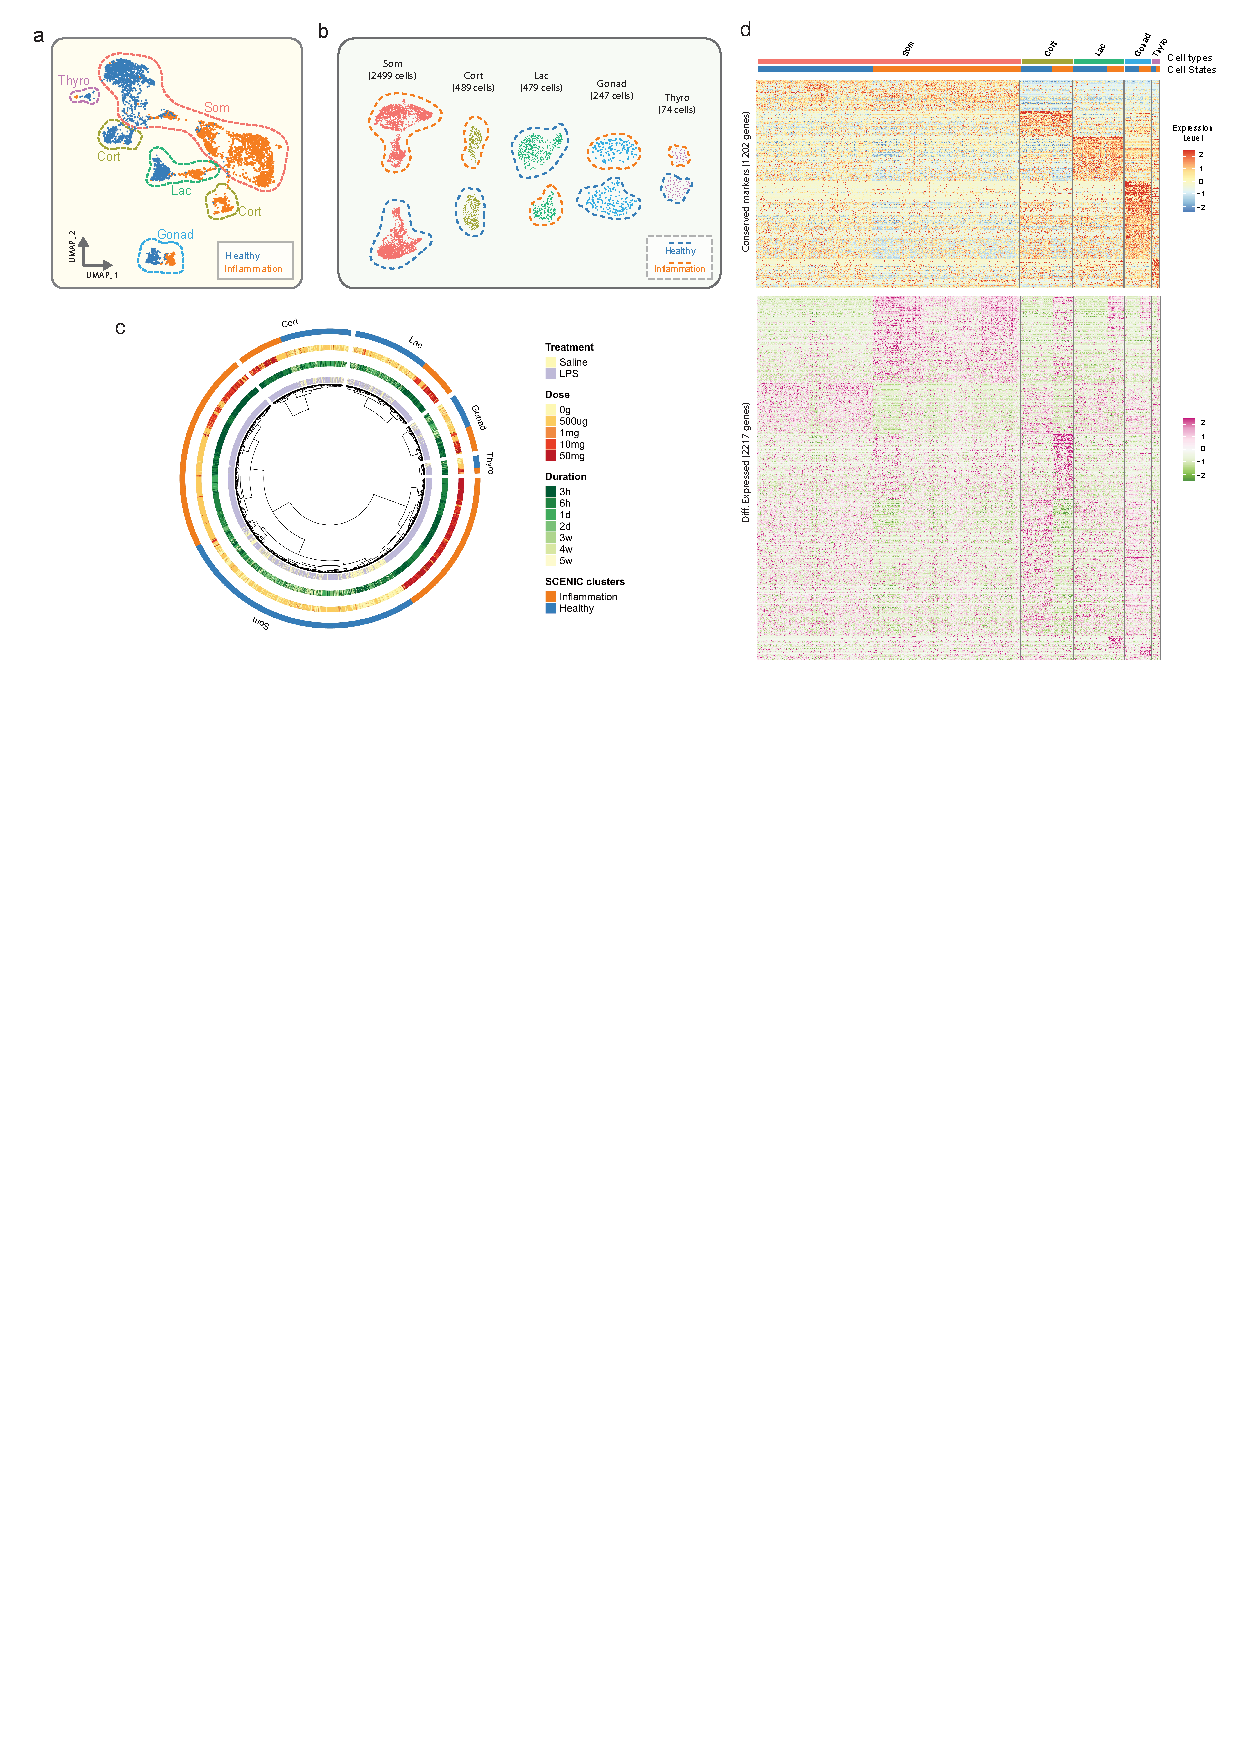
\includegraphics[width=1.0\textwidth]{figs/expr-fig2.pdf}
  \caption{单细胞测序数据SCENIC分析}
  \label{fig:expr-fig2}
\end{figure}

\subsection{分析处理条件与垂体细胞状态之间的关系}
  在我们所构建小鼠炎症模型中,我们依据免疫刺激剂、给药剂量与恢复时间尺度等因素建立了一系列实验。为了揭示这一系列因素与垂体细胞状态之间的关系,我们将这些处理条件与SCENIC聚类结果进行整合,如图\ref{fig:expr-fig2}c所示。

  我们可以看到所有注射saline的处理组,基本都处于健康(healthy)状态。除此之外,还有注射LPS的处理组也对应到了健康(healthy)状态。通过观察给药剂量与恢复时间尺度因素,我们可以发现这些细胞大多是注射低剂量LPS或者经历了长时程的恢复,在这种情况下神经系统仅有少量垂体细胞处于免疫应激状态。相比之下,注射高剂量LPS且仅经历短时程恢复的处理组则大多处于炎症(inflammation)状态。

\subsection{分析不同细胞在炎症状态下的基因表达差异}
  我们进一步比较了垂体中不同细胞在炎症状态下的基因表达差异,见图\ref{fig:expr-fig2}d。该图的上半部分是垂体各类细胞在其对应基因marker上的基因表达热图。同类细胞对应的基因marker无论中枢神经系统是否处于炎症状态,都会在该类细胞中稳定表达。然后,我们对每一类细胞分析其炎症状态与健康状态下的差异表达基因集合,并将其整合,便得到了该图的下半部分。

  我们发现同处于炎症状态,垂体中不同细胞应对炎症所做出的基因表达调整并不一致。例如,在炎症状态Somatotropes中上调最显著的基因集合并不是在炎症状态Corticotropes中上调最显著的基因集合。这便说明,在中枢神经内分泌系统处于炎症状态时,垂体内各类细胞会采取不同的应激方式,组成一个调节炎症反应的复杂系统。

\subsection{分析导致炎症状态的转录因子}
  我们依据SCENIC过程得到的AUC-score矩阵,统计出每个转录因子的AUC-score密度分布,我们希望找到具备双峰分布或者重尾分布的转录因子。对这些转录因子的分布进行自适应二值化,我们发现其标签可以和之前使用SCENIC聚类结果判定的细胞状态很好地匹配起来(见图\ref{fig:expr-fig3})。

  我们通过上面过程找到的转录因子涉及Stat、Irf以及Nfkb等转录因子家族,这些转录因子大多是与免疫过程相关的。例如,Irf7编码干扰素调节因子7,以往实验数据表明其在病毒诱导的细胞基因(包括I型干扰素基因)的转录中起作用。这些转录因子并没有像之前分析的差异表达基因那样展现出细胞种类特异性,而是在整个炎症状态的垂体细胞中广泛表达。

  这就表明Stat、Irf以及Nfkb等转录因子家族在垂体参与中枢神经内分泌炎症调节过程中扮演着重要的角色,影响着各类垂体细胞的调控路径。换句话说,Stat、Irf以及Nfkb等转录因子家族是垂体参与中枢神经内分泌炎症调节过程中的Master Regulator Genes(MRs)\cite{mattick2010global}。

\begin{figure}[!htb]
  \centering
  \includegraphics[width=0.8\textwidth]{figs/expr-fig3.pdf}
  \caption{具备双峰分布或者重尾分布的转录因子}
  \label{fig:expr-fig3}
\end{figure}

\section{讨论和未来工作}
  我们在实验中发现,在给以小鼠$TNF-\alpha$刺激之后,其部分垂体细胞在经历UMAP可视化降维之后,呈现出与其他炎症状态细胞相分离的现象。这似乎意味着垂体细胞在参与中枢神经内分泌炎症调节过程中,会因免疫刺激不同而进入不同的调节状态。

  我们初步推断是$TNF-\alpha$作为一种较强的免疫刺激剂,使垂体细胞进入一种不可逆转的免疫状态。在实验设计上,针对LPS、saline与Ploy I:C,我们都设计了长短恢复时程的对比试验,但$TNF-\alpha$只有短时程恢复处理。其原因在于$TNF-\alpha$相比LPS、Ploy I:C产生的免疫反应过于剧烈,小鼠在被腹腔注射500ug$TNF-\alpha$之后无法恢复,6h内便会死亡。

  我们未来的工作便打算在该研究的基础上,进一步探讨面对不可恢复炎症刺激与可恢复炎症刺激时垂体细胞在转录水平上的差异,揭示由健康(healthy)状态向这两种炎症(inflammation)状态转变的关键转录因子。



    %% end
    % ref
    % \nocite{*}
    \makebibliography
    % thanks
    %% thanks

\begin{acknowledgements}
  感谢蔡朝晖教授。她是大学期间为我们代课最多的老师,在我大学的学习成长过程和毕业论文撰写过程中提供了很大的指导和帮助。大一入学常听陈子轩和原昊博提起蔡老师,经过一段时间的接触,果然对学生十分负责!感谢蔡老师大学四年来对我的信任,让我在计算机本科学习中更加自信。

  感谢北京脑科学与类脑研究中心的罗敏敏教授。他在毕业论文撰写过程中给我提供了很大指导和帮助。我很敬佩罗老师对于科学的近乎狂热般的痴迷与对学生的关心。出于对神经科学的痴迷,我在保研的时候选择放弃我所擅长的计算机系统领域,转而投入神经科学领域。在刚保研完的时候,我深知我在神经科学领域的基础十分薄弱,便向罗老师申请到其实验室做毕设。罗老师并没有排斥一个本科其他专业的学生,而是在实验室本已满员的情况下十分认真地为我安排了一个相关方向的学长来指导我,让我更多地参与到实验室的课题中来,这为我以后从事神经科学领域研究打下了坚实的基础。

  与北京大学王睿宇学长的讨论让这篇论文更加完善。我们之后在神经科学领域会持续合作。

  感谢武汉大学的陈丹教授。大三上学期,选了他的一门专业选修课——计算机体系结构。陈老师在讲课的时候不拘泥于课本内容,而是十分注重培养我们的科研阅读素养。在与陈老师的交谈中,我了解到了很多体系结构前沿的研究,比如存内计算、类脑计算等,极大地开阔了我对于计算机系统的认识。也是通过陈老师的课,我对类脑计算、脑机接口与计算神经学等领域之间的联系有了初步的认知。最终走上科研道路、决定读博并且申请到北京大学前沿交叉学科研究院的PhD,陈老师起了巨大的引导作用。

  感谢武汉大学的艾浩军教授。大三下学期,由艾老师指导,和李蕴哲、朱赫合作完成的空中手写字符迁移学习项目最终成功发表,成为我人生中的第一篇论文!当时由于疫情,我们所有的交谈都被局限在线上。但艾老师每周都会与我们进行两小时以上的进展沟通,并对我们的工作提出建设性的指导意见。投稿前艾老师帮我们反复修改,在进行线上会议之前,他多次帮助我们修改海报以及展示视频,最终成功的展示离不开他的热心帮助。我们一直保持着联系。

  感谢浙江大学的潘纲教授。虽然接触的时间不长,但他的研究态度给我留下了深刻的印象——我们的电话交流永远发生在凌晨。实验室的博士生谭显瀚和祝歆韵日后都会是优秀的类脑计算研究者!这一段实习经历也让我更加坚定了从事神经科学研究的决心。

  感谢北京脑科学与类脑研究中心的周景峰教授,也是我未来的博士导师。在罗老师实验室便一直听说周师兄读博期间的各种经历,被实验室的师兄师姐一致称赞。之前在与他的交流中,我能深刻感受到他对于神经科学独到的理解与深厚的跨学科背景。虽然接触的时间还不长,但我能感受到他完美的性格!相信我们会有愉快、高产的合作。

  感谢北京生命科学联合中心的吴思教授和北京脑科学与类脑研究中心的柳昀哲教授。在与他们的交流中,我更加坚定了从神经元层级研究schema表示与修正过程的决心。我会在博士一年级到他们的实验室进行轮转。

  感谢北京生命科学研究所的王睿宇、卢立辉、袁正巍、刘志祥、曾佳为、黎亨、左鹏、于涛、全竞、严婷等同学。我十分享受与他们的每一次交流,他们对科学的严谨态度对我产生了深远的影响。

  感谢彭鹏、朱赫、李蕴哲、范文骞、章博文、周稚璇、陈子轩、原昊博等同学。感谢院学生会的同事们、WHU-MSC的朋友们、WHU-ICRobo的队友们,感谢所有的朋友。你们给我留下了永远的美好回忆!

  感谢武汉大学和弘毅学堂。学院“宽口径、厚基础、强能力”的教育方针,为我从事交叉学科的研究打下了坚实的基础。感谢弘毅学堂石兢、方萍、李瑶、董甲庆老师和辅导员王璐。

  感谢父母和家人长期的支持和鼓励。没有你们,我不会取得今天的成绩!

  四年的时光弹指一挥间,从青涩地踏进校园,到即将本科毕业,步入博士生涯。感谢过得飞快的时间,告诉我要不断努力,永不止步!

  最后用我很喜欢的一句话结束。感谢陈立杰的这句话。“能够生在这样一个黄金时代里,我感到无比的荣幸。我梦想能够成为黄金时代浪潮中的一朵浪花,为人类的智慧添砖加瓦!”
\end{acknowledgements}


    % appendix
    \include{pages/appendix}
\end{document}

